%!TEX root = ../thesis.tex
本研究で開発するロボットアームは,オープンプラットフォームとしての利用のしやすさを考慮し,オフィスロボットとして最低限の機能を要求する.本章では,従来のオフィスロボットのロボットアーム調査を行い,本研究で開発するロボットアームの要求仕様をまとめる.加えて,開発したロボットアームを検証する際に行う作業について,従来のオフィスロボットが対象としている作業を調査し検討する.
\section{ロボットアーム調査}
本節では,従来のオフィスロボットのロボットアーム20台を対象に,ロボットアームのメカニズムについて調査し,オフィスロボットのアームに最低限求められる機能をまとめる.

\subsection{アームリーチ}
従来のオフィスロボットのアームリーチ調査の結果(図\ref{fig:reach}参照),最小値は0.51m,最大値は0.90m,平均値および中央値はいずれも0.71mであった.この結果から,オフィス環境での作業には最低でも0.51m以上のアームリーチが必要であることが示唆される.さらに,調査対象10台中8台のロボットのアームリーチが0.75m以下であることから,0.75mを超えるアームリーチは現在のオフィスロボットが想定する作業には過剰である可能性が高い.

これらの結果に基づき,本研究ではアームリーチの要件を0.51mから0.75mの範囲に設定する.この範囲内のアームリーチであれば,基本的なオフィス作業に十分対応可能であると推測される.
\begin{figure}[h]
  \centering
  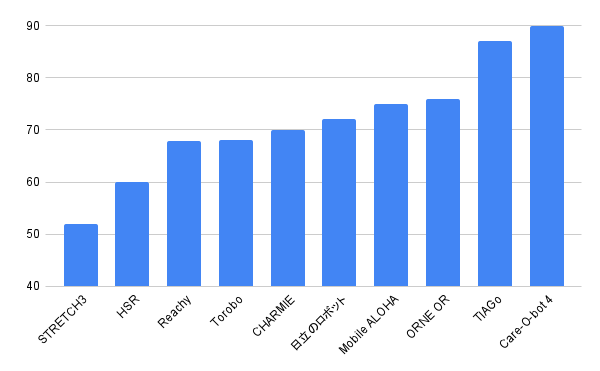
\includegraphics[width=10cm]{images/2syou/reach.png}
  \caption{Office robot arm reach survey results}
  \label{fig:reach}
\end{figure}

\subsection{可搬重量}
従来のオフィスロボットの可搬重量の最小は0.35kgであった(図\ref{fig:payload}参照).よって,現時点のオフィス作業においては0.5kg以上の可搬重量を確保できれば十分であると考えられるため,本研究では0.5kg以上を可搬重量の要件とした.
\begin{figure}
  \centering
  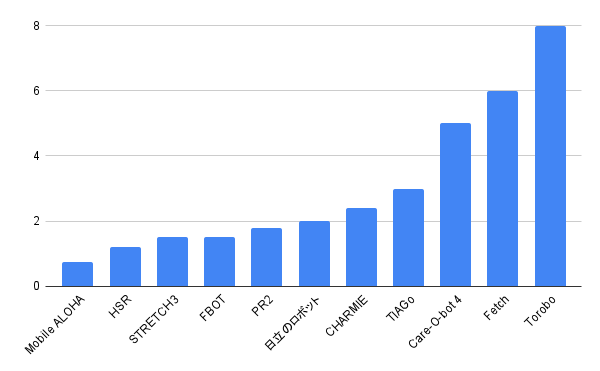
\includegraphics[width=10cm]{images/2syou/payload.png}
  \caption{Office robot payload survey results}
  \label{fig:payload}
\end{figure}
\clearpage

\subsection{自由度}
従来のオフィスロボットのアームの自由度を調査した結果,6自由度および7自由度のロボットが主流であることが確認された(図\ref{fig:armDof}参照).6自由度アームの典型的な軸配置は,肩2軸(ピッチ,ロール),肘1軸(ロール),手首3軸(ロール,ピッチ,ヨー)であり,7自由度アームでは肩に追加のロール軸が設けられている.7自由度アームは6自由度アームに比べて姿勢の自由度が増加する利点がある一方で,アーム重量やコストが増大する傾向がある.これらの要因を比較検討した結果,本研究ではコスト削減と軽量化を優先するため,6自由度アームを採用する.
\begin{figure}[h]
  \centering
  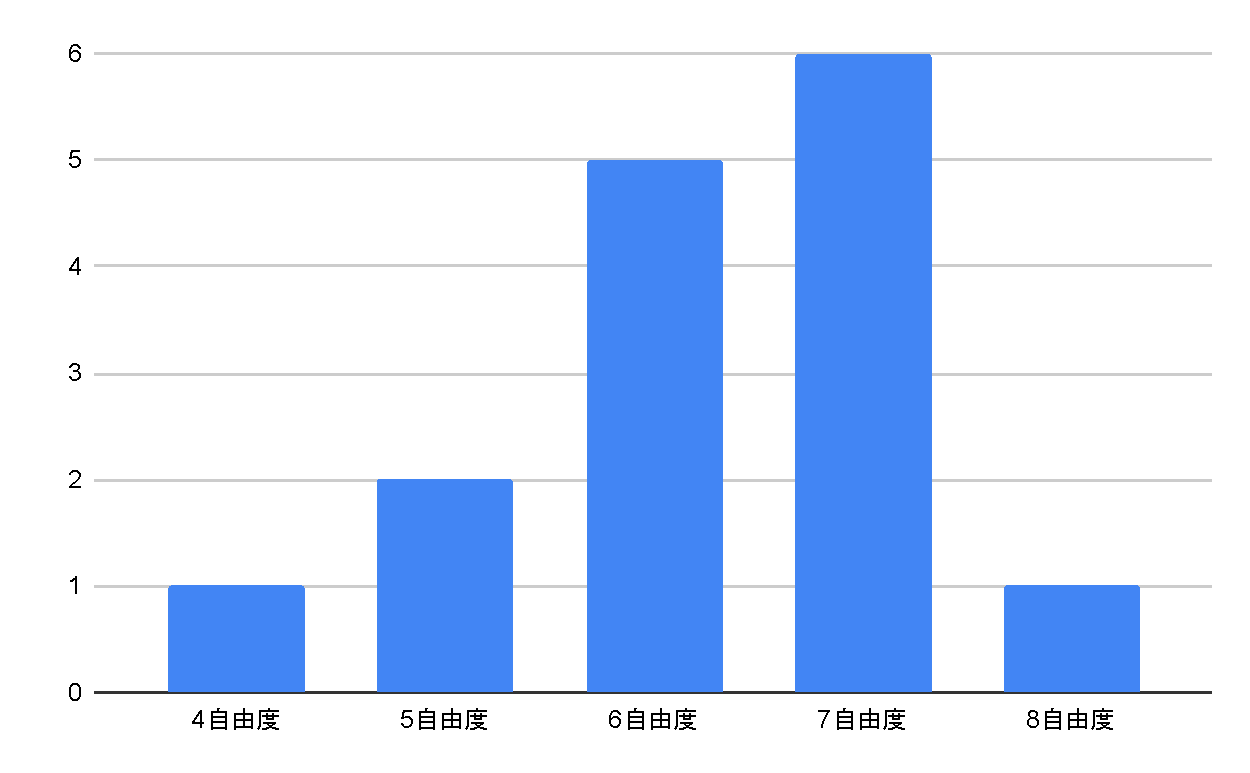
\includegraphics[width=10cm]{images/2syou/armDof.pdf}
  \caption{Office robot arm DoF survey results}
  \label{fig:armDof}
\end{figure}
\clearpage

\subsection{エンドエフェクタの形状}
従来のオフィスロボットで広く採用されているエンドエフェクタには,TIAGoに搭載されているような平行グリッパが挙げられる(図\ref{fig:tiago_hand}参照).PAL Robotics社が公開した動画\cite{TIAGo-movie:online}では,平行グリッパによって布,ジュース缶,スプレー缶,ジュースパック,板状物など,さまざまな形状の物体を把持する動作が示されている.オフィス作業において多様な形状の物体を確実に把持することが求められるため,本研究では,エンドエフェクタとして平行グリッパを採用する.
\begin{figure}[h]
  \centering
  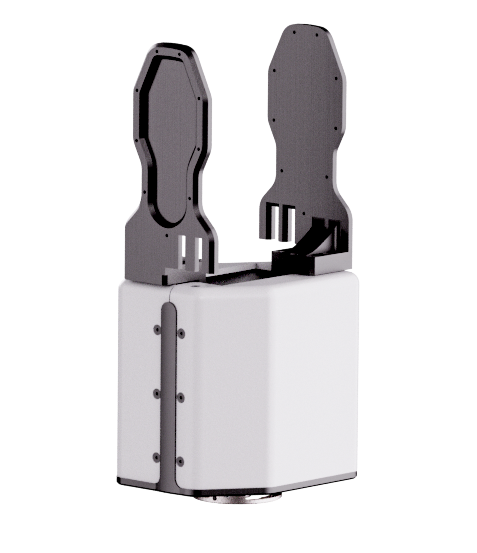
\includegraphics[width=8cm]{images/2syou/tiago_hand.png}
  \caption[End effectior of TIAGo]{End effectior of TIAGo (source: \cite{TIAGo:online})}
  \label{fig:tiago_hand}
\end{figure}
\clearpage

\subsection{オフィスロボットのロボットアームとして要求される項目}
以上を踏まえ,本研究で開発するロボットアームに,以下の項目を要求する.これを仕様として,ロボットアームのメカニズムを設計する.
\begin{itemize}
  \item 0.51m - 0.75mのアームリーチ
  \item 500g以上の可搬重量
  \item 6自由度アーム
  \item 平行グリッパのエンドエフェクタ
\end{itemize}
\newpage